% PKUMpLtX --- A LaTeX document class for 'Modern Physics Laboratory' in PKU based on `revtex4-2`
%
% Please read `README.md' and the template file before using
% 需要确保 font 选项指定的字体已安装! 具体参见 `README.md' 的说明.
\documentclass[font=default]{mpltx}

% 以下至 \begin{document} 都仅是本文件为了方便额外定义的命令, 写报告时不需要.
\hypersetup{colorlinks=true}% 超链接带颜色
\usepackage{xcolor}
\usepackage{tcolorbox}
\usepackage{enumitem}

\newtcbox{\buttombox}[1][red]
  {on line, arc = 3pt, outer arc = 3pt,
    colback = #1!10!white, colframe = #1!50!black,
    boxsep = 0pt, left = 2pt, right = 2pt, top = 1pt, bottom = 1pt,
    boxrule = 1pt}

\newcommand{\note}[1]{{\color{gray}#1}}
\NewDocumentCommand{\pkg}{s o m}{%
    \IfBooleanF{#1}{%
        \IfNoValueTF{#2}%
            {\href{https://www.ctan.org/pkg/#3}}%
            {\href{https://www.ctan.org/pkg/#2}}%
    }%
    {\textsf{#3}}%
}
\newcommand*\cs[1]{\texttt{\textbackslash #1}}
\newcommand*\env[1]{\textit{\texttt{#1}}}
\newcommand*\code[1]{\texttt{#1}}
\newcommand*\file[1]{\textbf{\texttt{#1}}}
\makeatletter
\newcommand\releasedate{%
    \href{https://github.com/CastleStar14654/PKUMpLtX/releases/tag/\mpltx@fileversion}%
        {\mpltx@filedate, \mpltx@fileversion}}
\makeatother
% 以上是本文件为了方便额外定义的命令, 写报告时不需要.

\begin{document}

\title{p 型硅的电阻率与霍尔系数随温度变化的研究} % 切合报告内容, 简短明确, 可以不同于讲义
\author{罗俊熙} % 这里 \emailphone 一定要紧跟在 \author 后方
\emailphone{see.looooo@stu.pku.edu.cn}{(86)13611162432}
% 如果改用 \email 则仅需要邮箱参数
\affiliation{北京大学物理学院\quad 学号: 2000012508}
% % 可以使用 \zhdate 自动生成中文日期, 如
% \date{\zhdate{2020/12/1}}
% % 也可使用 babel 的 \localedate, 如
% \date{\localedate{2020}{12}{1}}
% % 两者均会输出 `2020 年 12 月 1 日'
% 下面的 \date 的参数是为了自动输出正确版本号, 正式报告请替换为上面的两种 \date 之一
\date{\localedate{2023}{03}{18}}
\begin{abstract}
	测量半导体的电阻率与霍尔系数随温度变化的性质在研究中具有重要的地位。本研究使用范德堡法,在 $\qty{295}{\K}$ 到 $\qty{430}{\K}$ 的范围内测量了 p 型硅的电导率与霍尔系数,以及一系列的物理参量。利用内插的方法得到在 $\qty{300}{\K}$ 时半导体样品的电阻率为 $\qty{3553.6}{\ohm\per\cm}$,杂质浓度$N_A$为 $\qty{3.664e12}{\per\cubic\cm}$,样品的禁带宽度为 $\qty{1.21}{\eV}$。同时利用电阻率在不同温度区间的性质,得出本征激发区的温度大约在 $\qty{45}{\degreeCelsius}$ 以上。
\end{abstract}
\keywords{p 型硅半导体,范德堡法,霍尔系数}

\maketitle

\section{引言}
霍尔效应是与材料中的载流子在电场和磁场作用下所产生的效应有关的现象。1897年霍尔在研究导体在磁场中受力性质时发现,在电流与磁场垂直方向上有电势差。这个现象被称为霍尔效应。霍尔效应是半导体物理中一个重要的现象。通过测量在不同温度下体系的电阻率与霍尔系数,可以分析半导体材料中的杂质浓度、禁带宽度等一系列重要的物理量。因此,霍尔效应是一种重要的分析手段。

本研究的目的是通过在不同温度条件下对高阻 p 型硅的霍尔系数和电阻率的测量,了解半导体内存在本征导电以及杂质导电两种不同的导电机制。实验中使用范德堡法,测量从室温(约 $\qty{20}{\degreeCelsius}$)到 $\qty{160}{\degreeCelsius}$ 的温度区间内的 p 型硅半导体的电阻率以及霍尔系数。对比电阻率与霍尔系数随温度的变化规律,粗略估计杂质电离饱和区域与本征激发区的交界温度,并计算出 p 型硅半导体的禁带宽度 $E_g$、净杂质浓度 $N_A$、载流子浓度 p 与迁移率等一系列基本参量。
\section{实验目的}

\section{理论}\label{sec:theory}
\subsection{半导体作为光的增益介质}
电导率 $\sigma$ 与温度之间的关系如下图所示:

\begin{figure}[h]
\centering
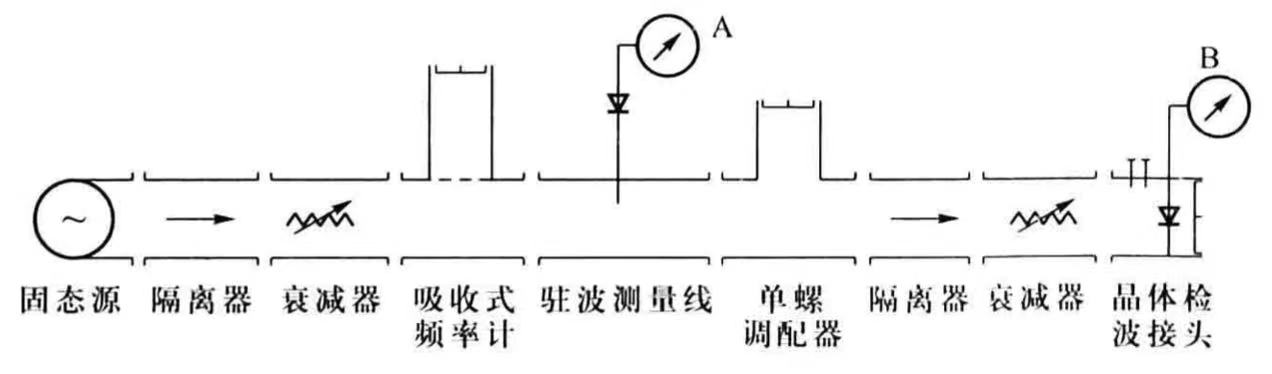
\includegraphics[width=0.6\textwidth]{fig/0.jpg}
\caption{电导率 $\sigma$ 与温度倒数 $1/T$ 的关系示意图}
\end{figure}

可以看到在不同温度下,半导体的电导率可以分成三个区域:
\begin{enumerate}
\item 杂质部分电离的温度区
\item 杂质电离饱和的温度区
\item 产生本征激发的高温区
\end{enumerate}

这三个区域分别对应着不同的导电机制\cite{jindaishiyan},在下面分别讨论:

\begin{enumerate}[label=\alph*) ]
	\item 杂质部分电离的温度区:在这个区域中,由杂质电离产生的载流子浓度随着温度上升而上升,同时载流子的迁移率也是取决于杂质散射。以上两个因素都是随着温度上升而增加,导致在杂质部份电离温度区中,电导率 $\sigma$ 随着温度上升而上升。

	\item 杂质电离饱和的温度区:在这个区域中,杂质已经被完全电离,但本征激发并不明显,导致载流子的浓度大致保持恒定。在这个温度下,迁移率主要取决于晶格散射,迁移率随着温度上升而下降,导致电导率 $\sigma$ 随温度上升而下降。
	在这个温度下,以 $300K$ 为基准,半导体材料的迁移率与电导率有以下的线性关系:
	\begin{equation}
		\mu_{Lp} = (\frac{\sigma}{\sigma_{300}})\mu_{Lp,300}
	\end{equation}
	其中,$\mu_{Lp,300}$ 与 $\sigma_{300}$ 分别对应着 $\qty{300}{\degreeCelsius}$ 下半导体材料的空穴迁移率与电导率,其中 ${\mu_{Lp,300}}=\qty{480}{\cm\squared\per\V\per\s}$。$\mu_{Lp,T}$ 与 $\sigma_T$ 分别对应着在杂质电离饱和区中不同温度的迁移率与电导率。

	\item 产生本征激发的高温区:这个区域中,由于本征激发产生的载流子随着温度上升而急剧上升,导致电导率在这个温度区间内会随着温度增加而急速上升。在这个区间之内,空穴载流子与电子的晶格散射迁移率,分别记为 $\mu_{Lp}$ 与 $\mu_{Ln}$,根据 Morin等人研究,迁移率与温度之间存在以下的幂次关系:
	
	\begin{equation}
		\mu_{Lp}(T) = 2.5\times10^9 T^{-2.3}\qty{}{\cm\squared\per\V\per\s}
	\end{equation}
	\begin{equation}
		\mu_{Ln}(T) = 4.0\times10^9 T^{-2.6}\qty{}{\cm\squared\per\V\per\s}
	\end{equation}

	同时,由半导体电中性条件得到:

	\begin{equation}
		p=(\frac{\sigma}{q\mu_{Lp}}+bp_s)/(b+1)
	\end{equation}
	\begin{equation}
		n=(\frac{\sigma}{q\mu_{Lp}}-p_s)/(b+1)
	\end{equation}
	
	其中,$b = \frac{\mu_{n}}{\mu_{p}}$,$p$ 与 $n$ 分别是空穴与电子的浓度。利用这两个物理量,可以决定半导体的禁带宽度:

	\begin{equation}
		E_g=\frac{k\Delta\ln(\frac{np}{T^3})}{\Delta(\frac{1}{T})}
	\end{equation}

	其中 $k$ 是玻尔兹曼常数。
\end{enumerate}

\subsection{霍尔效应}
对一个导体(或半导体)施加电流,同时在电流的垂直方向上施加磁场,在横向方向上会有一个电位差,称为霍尔电压 $V_H$,满足以下关系式:

$$V_H = \frac{R_H I B}{d}$$

其中,$R_H$ 是霍尔系数,$I$ 是施加的电流,$B$ 是与电流方向垂直的磁场,$d$ 是横向的距离。

如果体系是空穴与电子混合导电,并服从经典分布,在球状等能面的情况下,只考虑晶格散射与弱磁场近似,可以得到:

$$R_H = \frac{3\pi(p\mu_p^2 - n\mu_n^2)}{8q(p\mu_p + n\mu_n)^2}$$

从上式可以看到,霍尔系数与不同类型的载流子浓度有关,提示了可以通过霍尔系数来计算与载流子浓度相关的物理量。当 $R_H<0$ 时,对 $R_H$ 会出现一个极值点 $R^0_H$,有以下关系:

$$R^0_H = -\frac{3}{8}\frac{\pi N}{N_Aq}\frac{(b-1)^2}{4b}$$

\subsection{范德堡法测量任意形状薄片的电阻率及霍尔系数}
考虑一个任意形状、厚度为 $d$,没有孤立空洞的薄样品,如下图所示:
可以证明电阻率为:
\begin{equation}
\rho = \frac{\pi d}{\ln 2}\frac{R_{12,34} + R_{23,41}}{2}f
\end{equation}
其中,系数 $f$ 由以下方式决定:
\begin{equation}
\cosh{(\frac{R_{12,34}/R_{23,41}-1}{R_{12,34}/R_{23,41}+1}\cdot\frac{\ln2}{f})} = \frac{1}{2}\exp\left(\frac{\ln 2}{f}\right)
\end{equation}
其中,$R_{12,34}=\frac{V_4-V_3}{i_{12}}$,$R_{23,41}=\frac{V_1-V_4}{i_{23}}$,$i_{12}$、$i_{23}$、$i_{13}$ 为施加由$i$至$j$的电流。

如果接触点在样品四周边界上而且接触点足够小,样品厚度均匀而且没有空洞。在施加磁场后电流的分布与未施加磁场下电流的分布是一样的,利用这个特性,可以获得霍尔系数:
\begin{equation}
R_H=\frac{d}{B}\frac{\Delta(V_4-V_2)}{i_{13}}
\end{equation}
其中,$\Delta(V_4-V_2)$ 代表加磁场后 4 端与 2 端之间电位差的变化,$d$ 是样品厚度。
\section{实验装置及内容}
本次实验包含一个装有样品架的玻璃杜瓦瓶、永磁魔环、BWH-1 型霍耳效应测试仪、p 型硅片样本(电阻率大于$\qty{2500}{\ohm\cm}$)。
实验流程为
\begin{enumerate}
	\item 将样品放至永磁魔环中央,磁场方向和样品表面垂直,使魔环上标有$+B_m$的\buttombox[blue]{$\downarrow$}指向底盘上的\buttombox[red]{$\rightarrow$}位置。转动样品架,使样品表面法线方向与\buttombox[blue]{$\downarrow$}在同一本面内。
	\item 开启 BWH-1 型霍耳效应测试仪,同时打开\buttombox[blue]{样品温度}开关,打开\buttombox[blue]{恒流源},并使用$\qty{200}{\mA}$挡量程,通过控制永磁魔环和\buttombox[blue]{待测电压选择}旋钮测量出$\pm V_{\rm{I}}$,$\pm V_{\rm{II}}$,$V_{\rm{III}}(0,+I)$,$V_{\rm{III}}(0,-I)$,$V_{\rm{III}}(+B,+I)$,$V_{\rm{III}}(-B,-I)$。
	\item 测量和计算由室温到$\qty{165}{\degreeCelsius}$的电阻率和霍耳系数。
	\item 選做,在低溫條件下測量。
\end{enumerate}
\section{结果及讨论}
\subsubsection{半导体激光波长的标定}

\section{结论}

% bibliography 的参数是你的 *.bib 文件去掉后缀名后的部分
\bibliography{bibli}

\clearpage % 附录前另起一页
\appendix % 附录开始
\section{思考题}\label{app:exercise}
\subsection{为甚么实验失败?}

\end{document}
